\documentclass{beamer}
\usetheme{default}
\usecolortheme{default}
\setbeamertemplate{navigation symbols}{}
\setbeamertemplate{footline}[frame number]

\usepackage{amsmath,amssymb}
\usepackage{graphicx}
\usepackage{booktabs}
\usepackage{xcolor}
\usepackage{tikz}
\usepackage{pgfplots}
\pgfplotsset{compat=1.18}
\usetikzlibrary{shapes.geometric, arrows.meta, positioning, calc, patterns, decorations.pathreplacing}
\usepackage{adjustbox}
\usepackage{array}
\usepackage{multicol}
\setlength{\tabcolsep}{3pt}

\definecolor{darkblue}{RGB}{0,51,102}
\definecolor{lightgray}{RGB}{240,240,240}
\definecolor{rlgreen}{RGB}{52,211,153}
\definecolor{tradred}{RGB}{255,107,107}
\definecolor{hpapurp}{RGB}{192,132,252}
\definecolor{seeryel}{RGB}{252,211,77}
\definecolor{openfaas}{RGB}{255,165,0}
\definecolor{sparkred}{RGB}{230,76,60}
\definecolor{kafkapurp}{RGB}{120,80,180}
\definecolor{edgeblue}{RGB}{96,165,250}

\setbeamercolor{frametitle}{fg=darkblue,bg=lightgray}
\setbeamercolor{title}{fg=darkblue}
\setbeamercolor{structure}{fg=darkblue}

\title[Serverless Spark IoT Framework]{\textbf{Serverless Spark Framework for Real-Time IoT Applications}\\[6pt]
\small{With Hierarchical RL \& OpenFaaS Serverless Orchestration}}
\author{Naman Rao \and Manvith M \and Kancharla Rohan \and Nithin Reddy}
\institute{Indian Institute of Information Technology, Kottayam}
\date{Final Review --- \today}

\begin{document}

% ===================================================================
% SLIDE 1: Title
% ===================================================================
\begin{frame}
\titlepage
\begin{center}
\small{Guided by: \textbf{Dr.\ Shajulin Benedict}}
\end{center}
\end{frame}

% ===================================================================
% SLIDE 2: Outline
% ===================================================================
\begin{frame}{Outline}
\tableofcontents
\end{frame}

% ===================================================================
\section{Introduction}
% ===================================================================

% SLIDE 3
\begin{frame}{Introduction}
\begin{itemize}
    \item IoT devices generate continuous, high-volume data requiring \textbf{sub-second} analysis.
    \item Apache Spark is efficient for distributed processing but relies on \textbf{static configuration}.
    \item Traditional auto-scalers (HPA, linear predictors) are \textbf{reactive} --- they respond \textit{after} the spike.
    \item Our framework automates scaling using \textbf{Two-Phase Hierarchical Reinforcement Learning}.
\end{itemize}
\vspace{0.3cm}
\begin{block}{Goal}
Achieve real-time IoT processing with minimal cost and latency using an intelligent, \textbf{proactive} optimizer deployed as an \textbf{OpenFaaS serverless function}.
\end{block}
\end{frame}

% SLIDE 4
\begin{frame}{Problem Statement}
\begin{block}{Research Question}
How can a Spark-based IoT framework process highly variable workloads efficiently---balancing throughput, latency, and cost---without manual intervention?
\end{block}
\vspace{0.3cm}
\textbf{Objectives:}
\begin{enumerate}
    \item Build an IoT-to-Spark pipeline using MQTT and Kafka.
    \item Implement a \textbf{Two-Phase RL system} (PPO + TD3) for dynamic resource allocation.
    \item Deploy the RL decision engine as an \textbf{OpenFaaS serverless function}.
    \item Integrate \textbf{edge-aware cold start mitigation} with pattern-based pre-warming.
    \item Implement \textbf{adaptive shuffle storage tiering} (Redis / SSD / S3).
\end{enumerate}
\end{frame}

% ===================================================================
\section{Literature Review}
% ===================================================================

% SLIDE 5
\begin{frame}{Existing Systems \& Research Gap}
\begin{table}
\footnotesize
\begin{tabular}{|l|l|l|l|}
\hline
\textbf{Framework} & \textbf{Year} & \textbf{Approach} & \textbf{Limitation} \\
\hline
Seer & 2022 & 2-tier shuffle optimization & Static, not IoT-focused \\
Dexter & 2024 & Linear regression model & Single objective only \\
SPSC & 2024 & Lambda-based stream engine & Not Spark-compatible \\
Laminar 2.0 & 2024 & Recomputational pipeline & No adaptive tuning \\
ServerlessYarn & 2024 & Container orchestration & Not fully serverless \\
\hline
\end{tabular}
\end{table}
\vspace{0.3cm}
\begin{alertblock}{Gap Identified}
No existing framework combines: (1) Multi-objective RL, (2) Serverless function deployment, (3) Edge-aware proactive scaling, and (4) Adaptive storage tiering --- in a single system.
\end{alertblock}
\end{frame}

% ===================================================================
\section{System Architecture}
% ===================================================================

% SLIDE 6
\begin{frame}{5-Layer System Architecture}
\centering
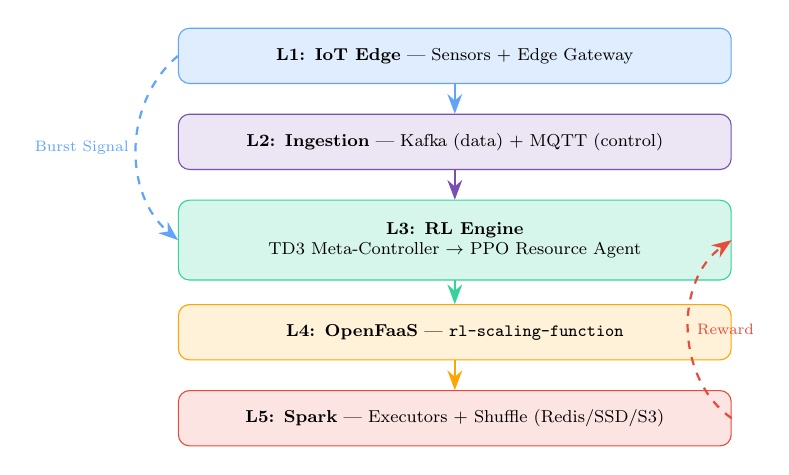
\begin{tikzpicture}[
    layer/.style={rectangle, draw, rounded corners=4pt, minimum width=9cm, minimum height=0.9cm, font=\footnotesize, align=center},
    arr/.style={-{Stealth[length=2.5mm]}, thick},
    scale=0.78, transform shape
]
\node[layer, fill=edgeblue!20, draw=edgeblue] (L1) at (0,5.2) {\textbf{L1: IoT Edge} --- Sensors + Edge Gateway};
\node[layer, fill=kafkapurp!15, draw=kafkapurp] (L2) at (0,3.8) {\textbf{L2: Ingestion} --- Kafka (data) + MQTT (control)};
\node[layer, fill=rlgreen!20, draw=rlgreen, minimum height=1.3cm] (L3) at (0,2.2) {\textbf{L3: RL Engine}\\TD3 Meta-Controller $\rightarrow$ PPO Resource Agent};
\node[layer, fill=openfaas!15, draw=openfaas] (L4) at (0,0.7) {\textbf{L4: OpenFaaS} --- \texttt{rl-scaling-function}};
\node[layer, fill=sparkred!15, draw=sparkred] (L5) at (0,-0.7) {\textbf{L5: Spark} --- Executors + Shuffle (Redis/SSD/S3)};

\draw[arr, edgeblue] (L1) -- (L2);
\draw[arr, kafkapurp] (L2) -- (L3);
\draw[arr, rlgreen] (L3) -- (L4);
\draw[arr, openfaas] (L4) -- (L5);
\draw[arr, sparkred, dashed] (L5.east) to[bend left=55] node[right, font=\scriptsize] {Reward} (L3.east);
\draw[arr, edgeblue, dashed] (L1.west) to[bend right=50] node[left, font=\scriptsize] {Burst Signal} (L3.west);
\end{tikzpicture}
\end{frame}

% SLIDE 7
\begin{frame}{Data Flow: End-to-End Pipeline}
\centering
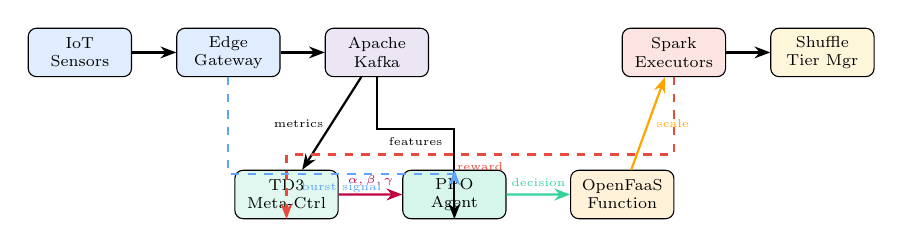
\begin{tikzpicture}[
    box/.style={rectangle, draw, rounded corners=3pt, minimum height=0.75cm, font=\scriptsize, align=center, minimum width=1.6cm},
    arr/.style={-{Stealth[length=2mm]}, thick},
    scale=0.82, transform shape
]
% Top row: data path
\node[box, fill=edgeblue!20] (iot)   at (0,0)     {IoT\\Sensors};
\node[box, fill=edgeblue!20] (edge)  at (2.3,0)   {Edge\\Gateway};
\node[box, fill=kafkapurp!15](kafka) at (4.6,0)   {Apache\\Kafka};
\node[box, fill=sparkred!15] (spark) at (9.2,0)   {Spark\\Executors};
\node[box, fill=seeryel!20]  (shuf)  at (11.5,0)  {Shuffle\\Tier Mgr};

% Bottom row: RL + OpenFaaS
\node[box, fill=rlgreen!15]  (meta)  at (3.2,-2.2) {TD3\\Meta-Ctrl};
\node[box, fill=rlgreen!20]  (ppo)   at (5.8,-2.2) {PPO\\Agent};
\node[box, fill=openfaas!15] (faas)  at (8.4,-2.2) {OpenFaaS\\Function};

% Data path arrows
\draw[arr] (iot) -- (edge);
\draw[arr] (edge) -- (kafka);
\draw[arr] (spark) -- (shuf);

% Kafka to RL
\draw[arr] (kafka) -- node[left, font=\tiny]{metrics} (meta);
\draw[arr, purple] (meta) -- node[above, font=\tiny]{$\alpha,\beta,\gamma$} (ppo);
\draw[arr] (kafka.south) -- ++(0,-0.8) -| node[below, font=\tiny, near start]{features} (ppo.south);

% RL to Spark via OpenFaaS
\draw[arr, rlgreen] (ppo) -- node[above, font=\tiny]{decision} (faas);
\draw[arr, openfaas] (faas) -- node[right, font=\tiny]{scale} (spark);

% Feedback loops
\draw[arr, dashed, sparkred] (spark.south) -- ++(0,-1.2) -| node[below, font=\tiny, near start]{reward} (meta.south);
\draw[arr, dashed, edgeblue] (edge.south) -- ++(0,-1.5) -| node[below, font=\tiny, near start]{burst signal} (ppo);
\end{tikzpicture}
\end{frame}

% SLIDE 8
\begin{frame}{Ingestion Layer: MQTT + Kafka}
\textbf{Dual-Lane Architecture:}
\[ \text{IoT Sensors} \xrightarrow{\text{MQTT}} \text{Edge Gateway} \xrightarrow{\text{Kafka}} \text{Spark Streaming} \]

\vspace{0.2cm}
\begin{columns}
\column{0.48\textwidth}
\textbf{High-Throughput Lane (Kafka):}
\begin{itemize}
    \item Bulk telemetry data at scale
    \item Durable, replayable
    \item Partitioned for parallelism
\end{itemize}

\column{0.48\textwidth}
\textbf{Low-Latency Control Lane (MQTT):}
\begin{itemize}
    \item Edge burst signals
    \item RL state updates
    \item Lightweight, sub-10ms
\end{itemize}
\end{columns}
\vspace{0.3cm}
\textbf{Why Both?} Separating data from control traffic ensures scaling decisions are never delayed by a congested data pipeline.
\end{frame}

% SLIDE 9
\begin{frame}{Processing Layer: Serverless Spark}
\textbf{Serverless Execution Model:}
\begin{itemize}
    \item Spark jobs run as ephemeral containers.
    \item \textbf{Challenge:} Cold start delays (45--60s to boot new executors).
    \item \textbf{Solution:} RL agent \textbf{pre-emptively} scales executors using edge burst prediction.
\end{itemize}
\vspace{0.3cm}
\textbf{Integration:}
\begin{itemize}
    \item Spark Structured Streaming with \texttt{foreachBatch}.
    \item Continuous metric collection (Latency, Throughput, Cost) fed to RL.
    \item \textbf{Adaptive Shuffle:} Dynamic storage tier selection based on data temperature.
\end{itemize}
\end{frame}

% ===================================================================
\section{Phase 1: PPO Scaling Agent}
% ===================================================================

% SLIDE 10
\begin{frame}{Phase 1: PPO Scaling Agent --- Tactical Decisions}
\textbf{Goal:} Optimize immediate resource allocation every $\sim$5 seconds.

\vspace{0.2cm}
\textbf{State Space (20 Dimensions):}
\begin{itemize}
    \item 13 base: Workload rate, CPU, Memory, Latency, Cost, $\alpha$, $\beta$, $\gamma$, shuffle size, data temperature, edge signals
    \item 7 pattern features: velocity, acceleration, rolling mean/std, burst probability, hour encoding
\end{itemize}

\textbf{Action Space:} \texttt{SCALE\_UP}, \texttt{SCALE\_DOWN}, \texttt{MAINTAIN}, \texttt{PRE\_WARM}

\vspace{0.2cm}
\textbf{Reward Function (Dynamic Weights from Phase 2):}
\[ R = -\alpha \cdot C_{\text{norm}} - \beta \cdot L_{\text{norm}} + \gamma \cdot T_{\text{norm}} + R_{\text{cold\_start}} \]
\end{frame}

% SLIDE 11
\begin{frame}{Phase 1: PPO Training Results}
\centering
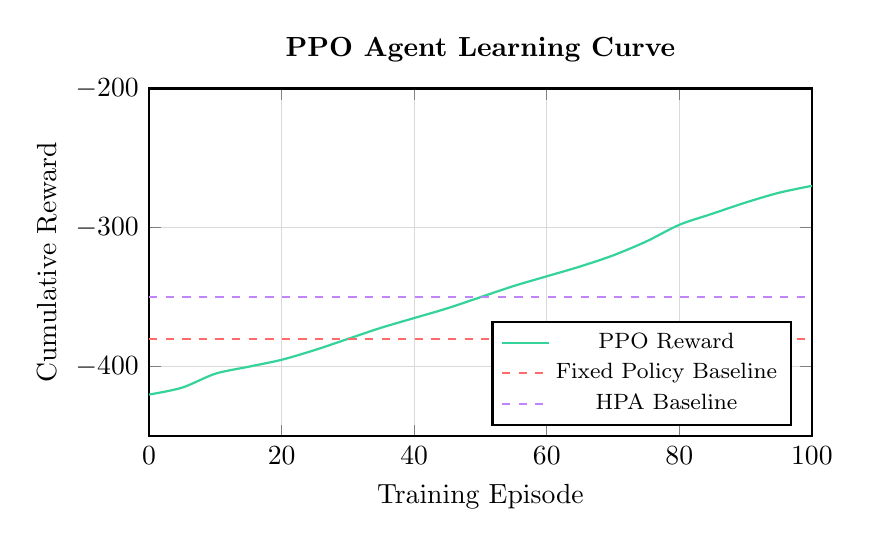
\begin{tikzpicture}
\begin{axis}[
    width=10cm, height=6cm,
    xlabel={Training Episode}, ylabel={Cumulative Reward},
    title={\textbf{PPO Agent Learning Curve}},
    grid=major, grid style={gray!30},
    ymin=-450, ymax=-200,
    xmin=0, xmax=100,
    thick,
    legend pos=south east,
    legend style={font=\footnotesize}
]
\addplot[rlgreen, thick, smooth] coordinates {
    (0,-420)(5,-415)(10,-405)(15,-400)(20,-395)
    (25,-388)(30,-380)(35,-372)(40,-365)(45,-358)
    (50,-350)(55,-342)(60,-335)(65,-328)(70,-320)
    (75,-310)(80,-298)(85,-290)(90,-282)(95,-275)(100,-270)
};
\addlegendentry{PPO Reward}
\addplot[tradred, dashed, thick] coordinates {(0,-380)(100,-380)};
\addlegendentry{Fixed Policy Baseline}
\addplot[hpapurp, dashed, thick] coordinates {(0,-350)(100,-350)};
\addlegendentry{HPA Baseline}
\end{axis}
\end{tikzpicture}
\vspace{0.2cm}

Agent converges after $\sim$80 episodes. Surpasses both baselines by Episode 40.
\end{frame}

% SLIDE 12
\begin{frame}{Phase 1: RL Decision Demo (3 Scenarios)}
\begin{table}[H]
\centering
\scriptsize
\begin{tabular}{|l|c|c|c|}
\hline
\textbf{Parameter} & \textbf{High Load} & \textbf{Moderate} & \textbf{Low Load} \\
 & 450 msg/s & 150 msg/s & 30 msg/s \\
\hline
Action & SCALE\_UP & MAINTAIN & SCALE\_DOWN \\
Executors & 17 & 8 & 2 \\
Storage Tier & HOT (Redis) & WARM (SSD) & COLD (S3) \\
Cost & \$6.90/hr & \$4.00/hr & \$1.00/hr \\
Latency & 87 ms & 195 ms & 450 ms \\
Throughput & 118 u/s & 46 u/s & 12 u/s \\
\hline
\end{tabular}
\end{table}
\vspace{0.2cm}
\begin{alertblock}{Phase 1 Limitation}
Uses fixed weights ($\alpha{=}0.4, \beta{=}0.4, \gamma{=}0.2$). Cannot adapt priorities when workload context changes (e.g., budget crunch vs.\ healthcare emergency).
\end{alertblock}
$\Rightarrow$ \textbf{Need for Phase 2: Meta-Controller.}
\end{frame}

% ===================================================================
\section{Phase 2: TD3 Meta-Controller}
% ===================================================================

% SLIDE 13
\begin{frame}{Phase 2: Two-RL Hierarchical Architecture}
\centering
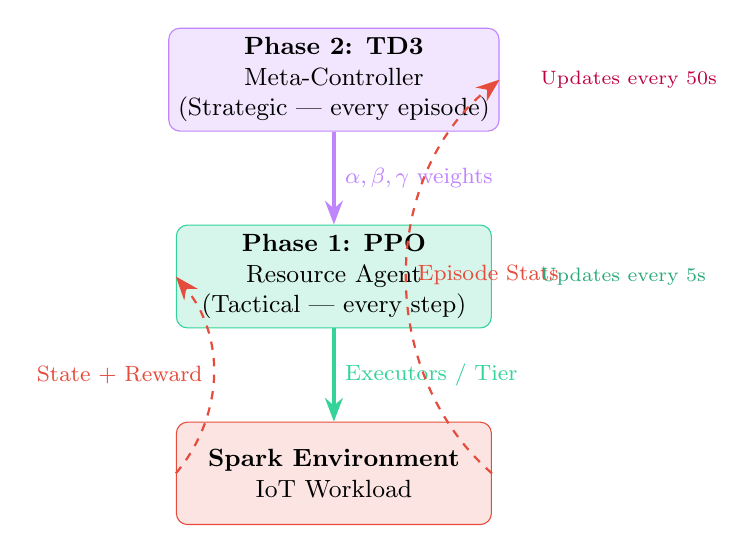
\begin{tikzpicture}[
    box/.style={rectangle, draw, rounded corners=4pt, minimum width=4cm, minimum height=1.3cm, align=center, font=\small},
    arr/.style={-{Stealth[length=3mm]}, thick},
]
\node[box, fill=hpapurp!20, draw=hpapurp] (td3) at (0,3) {\textbf{Phase 2: TD3}\\Meta-Controller\\(Strategic --- every episode)};
\node[box, fill=rlgreen!20, draw=rlgreen] (ppo) at (0,0.5) {\textbf{Phase 1: PPO}\\Resource Agent\\(Tactical --- every step)};
\node[box, fill=sparkred!15, draw=sparkred] (env) at (0,-2) {\textbf{Spark Environment}\\IoT Workload};

\draw[arr, hpapurp, line width=1.5pt] (td3) -- node[right, font=\footnotesize] {$\alpha, \beta, \gamma$ weights} (ppo);
\draw[arr, rlgreen, line width=1.5pt] (ppo) -- node[right, font=\footnotesize] {Executors / Tier} (env);
\draw[arr, sparkred, dashed] (env.west) to[bend right=40] node[left, font=\footnotesize] {State + Reward} (ppo.west);
\draw[arr, sparkred, dashed] (env.east) to[bend left=50] node[right, font=\footnotesize] {Episode Stats} (td3.east);

\node[font=\scriptsize, text=purple, right] at (2.5,3) {Updates every 50s};
\node[font=\scriptsize, text=rlgreen!80!black, right] at (2.5,0.5) {Updates every 5s};
\end{tikzpicture}
\end{frame}

% SLIDE 14
\begin{frame}{Phase 2: TD3 Algorithm}
\textbf{Why TD3 (Twin Delayed DDPG)?}
\begin{itemize}
    \item \textbf{Continuous control:} Outputs precise weights (e.g., $\alpha{=}0.345$).
    \item \textbf{Twin critics} prevent reward overestimation.
    \item \textbf{Delayed updates} improve training stability.
\end{itemize}
\vspace{0.2cm}
\textbf{State Space (9-dim):} Hour, day, business hours, latency ratio, cost ratio, throughput ratio, SLA violation rate, latency trend, cost trend.

\vspace{0.1cm}
\textbf{Action Space:} $\alpha, \beta, \gamma \in \mathbb{R}^3 \xrightarrow{\text{softmax}} \alpha+\beta+\gamma=1$

\vspace{0.1cm}
\textbf{Meta-Reward:}
\[ R_{\text{meta}} = \underbrace{R_{\text{SLA}}}_{\text{latency compliance}} + \underbrace{R_{\text{budget}}}_{\text{cost compliance}} - 0.5 \times V_{\text{violations}} + 0.2 \times R_{\text{stability}} \]
\end{frame}

% SLIDE 15
\begin{frame}{Phase 2: Adaptive Weight Learning}
\centering
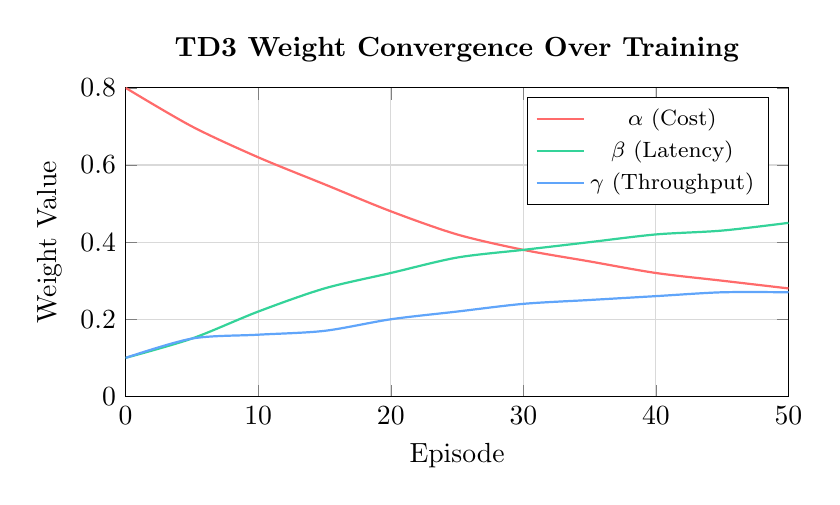
\begin{tikzpicture}
\begin{axis}[
    width=10cm, height=5.5cm,
    xlabel={Episode}, ylabel={Weight Value},
    title={\textbf{TD3 Weight Convergence Over Training}},
    grid=major, grid style={gray!30},
    ymin=0, ymax=0.8,
    xmin=0, xmax=50,
    legend pos=north east,
    legend style={font=\footnotesize}
]
\addplot[tradred, thick, smooth] coordinates {
    (0,0.8)(5,0.7)(10,0.62)(15,0.55)(20,0.48)(25,0.42)
    (30,0.38)(35,0.35)(40,0.32)(45,0.30)(50,0.28)
};
\addlegendentry{$\alpha$ (Cost)}
\addplot[rlgreen, thick, smooth] coordinates {
    (0,0.1)(5,0.15)(10,0.22)(15,0.28)(20,0.32)(25,0.36)
    (30,0.38)(35,0.40)(40,0.42)(45,0.43)(50,0.45)
};
\addlegendentry{$\beta$ (Latency)}
\addplot[edgeblue, thick, smooth] coordinates {
    (0,0.1)(5,0.15)(10,0.16)(15,0.17)(20,0.20)(25,0.22)
    (30,0.24)(35,0.25)(40,0.26)(45,0.27)(50,0.27)
};
\addlegendentry{$\gamma$ (Throughput)}
\end{axis}
\end{tikzpicture}
\vspace{0.2cm}

TD3 learns to shift from cost-heavy ($\alpha{=}0.8$) to a balanced latency-priority policy.
\end{frame}

% SLIDE 16
\begin{frame}{Adaptive Behaviour: Burst Response Demo}
\begin{columns}
\column{0.48\textwidth}
\textbf{Step 1: Latency Spike Detected}
\begin{itemize}
    \item Latency $>$ 200ms
    \item SLA violation imminent
\end{itemize}
\textbf{Step 2: TD3 Reacts}
\begin{itemize}
    \item $\alpha \downarrow 0.1$ (ignore cost)
    \item $\beta \uparrow 0.8$ (maximize speed)
\end{itemize}

\column{0.48\textwidth}
\textbf{Step 3: PPO Executes}
\begin{itemize}
    \item Sees new weights ($\beta{=}0.8$)
    \item \textbf{Action:} Aggressive \texttt{SCALE\_UP}
    \item +4 executors, Redis HOT tier
\end{itemize}
\textbf{Result:}
\begin{itemize}
    \item Latency: 210ms $\rightarrow$ 87ms
    \item SLA preserved
    \item Cost resumes after spike
\end{itemize}
\end{columns}
\end{frame}

% ===================================================================
\section{OpenFaaS Integration}
% ===================================================================

% SLIDE 17
\begin{frame}{OpenFaaS: Serverless RL Deployment}
\textbf{Why OpenFaaS?}
\begin{itemize}
    \item Decouples the RL ``brain'' from Spark --- independently scalable.
    \item Event-driven: invoked only when metrics arrive (no idle cost).
    \item Enables \textbf{scale-to-zero}: the optimizer itself is serverless.
\end{itemize}
\vspace{0.2cm}
\centering
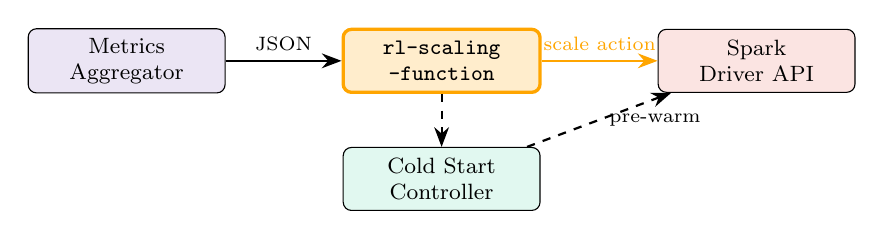
\begin{tikzpicture}[
    box/.style={rectangle, draw, rounded corners=3pt, minimum height=0.8cm, font=\footnotesize, align=center, minimum width=2.5cm},
    arr/.style={-{Stealth[length=2.5mm]}, thick},
]
\node[box, fill=kafkapurp!15] (metrics) at (0,0) {Metrics\\Aggregator};
\node[box, fill=openfaas!20, draw=openfaas, line width=1.2pt] (faas) at (4,0) {\texttt{rl-scaling}\\\texttt{-function}};
\node[box, fill=sparkred!15] (spark) at (8,0) {Spark\\Driver API};
\node[box, fill=rlgreen!15] (cold) at (4,-1.5) {Cold Start\\Controller};

\draw[arr] (metrics) -- node[above, font=\scriptsize]{JSON} (faas);
\draw[arr, openfaas] (faas) -- node[above, font=\scriptsize]{scale action} (spark);
\draw[arr, dashed] (faas) -- (cold);
\draw[arr, dashed] (cold) -- node[right, font=\scriptsize]{pre-warm} (spark);
\end{tikzpicture}
\end{frame}

% SLIDE 18
\begin{frame}{OpenFaaS: Request/Response Format}
\textbf{Request (JSON):}
\begin{center}
\footnotesize
\texttt{\{"workload\_rate": 300, "cpu\_util": 82, "edge\_burst\_signal": 0.85,}\\
\texttt{~~"alpha": 0.15, "beta": 0.70, "burst\_probability": 0.72\}}
\end{center}
\vspace{0.2cm}
\textbf{Response:}
\begin{center}
\footnotesize
\texttt{\{"action": "pre\_warm", "target\_executors": 12,}\\
\texttt{~~"pre\_warm\_count": 6, "confidence": 0.92\}}
\end{center}
\vspace{0.3cm}
\textbf{Decision Priority Logic:}
\begin{enumerate}
    \footnotesize
    \item Very low load $\rightarrow$ \texttt{scale\_to\_zero} (true serverless idle)
    \item Pattern burst detected (burst\_prob $>$ 0.6) $\rightarrow$ \texttt{pre\_warm}
    \item Edge burst signal ($>$ 0.5) $\rightarrow$ \texttt{pre\_warm}
    \item High load / CPU $\rightarrow$ \texttt{scale\_up}
    \item Cost-sensitive + moderate load $\rightarrow$ \texttt{scale\_down}
\end{enumerate}
\end{frame}

% ===================================================================
\section{Cold Start Mitigation}
% ===================================================================

% SLIDE 19
\begin{frame}{Cold Start Problem \& Solution}
\textbf{The Problem:} Booting new Spark executors takes 45--60 seconds.\\
By the time reactive scalers detect a spike, the SLA is already breached.

\vspace{0.3cm}
\textbf{Our Solution --- Pattern-Aware Pre-Warming:}
\centering
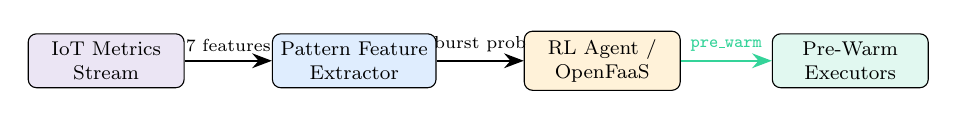
\begin{tikzpicture}[
    box/.style={rectangle, draw, rounded corners=3pt, minimum height=0.7cm, font=\footnotesize, align=center, minimum width=2.2cm},
    arr/.style={-{Stealth[length=2.5mm]}, thick},
    scale=0.9, transform shape
]
\node[box, fill=kafkapurp!15] (stream) at (0,0) {IoT Metrics\\Stream};
\node[box, fill=edgeblue!20] (pfe) at (3.5,0) {Pattern Feature\\Extractor};
\node[box, fill=openfaas!15] (rl) at (7,0) {RL Agent /\\OpenFaaS};
\node[box, fill=rlgreen!15] (pre) at (10.5,0) {Pre-Warm\\Executors};

\draw[arr] (stream) -- node[above, font=\scriptsize]{7 features} (pfe);
\draw[arr] (pfe) -- node[above, font=\scriptsize]{burst prob} (rl);
\draw[arr, rlgreen] (rl) -- node[above, font=\scriptsize]{\texttt{pre\_warm}} (pre);
\end{tikzpicture}

\vspace{0.3cm}
\textbf{7 Pattern Features:}
\begin{multicols}{2}
\footnotesize
\begin{enumerate}
    \item Traffic velocity
    \item Traffic acceleration
    \item Rolling mean
    \item Rolling std
    \item Burst probability
    \item Hour sine encoding
    \item Hour cosine encoding
\end{enumerate}
\end{multicols}
\end{frame}

% SLIDE 20
\begin{frame}{Adaptive Shuffle Storage Tiering}
\textbf{Spark's shuffle} is the primary performance bottleneck. We replace the default single-tier with RL-driven dynamic tier selection.

\vspace{0.3cm}
\begin{table}[H]
\centering
\footnotesize
\begin{tabular}{|c|l|c|c|l|}
\hline
\textbf{Tier} & \textbf{Backend} & \textbf{Latency} & \textbf{Cost} & \textbf{Best For} \\
\hline
\textcolor{red}{\textbf{HOT}} & Redis (in-memory) & $\sim$50 $\mu$s & Highest & Bursts, iterative ML \\
\textcolor{orange}{\textbf{WARM}} & NVMe SSD & $\sim$200 $\mu$s & Moderate & Standard ETL \\
\textcolor{gray}{\textbf{COLD}} & S3 / HDD & $\sim$5 ms & Lowest & Batch, archival \\
\hline
\end{tabular}
\end{table}

\vspace{0.2cm}
\begin{exampleblock}{Result}
RL classifies each data batch by reuse probability and assigns the optimal tier.\\
\textbf{2.8$\times$ throughput improvement} with Redis HOT tier during bursts.
\end{exampleblock}
\end{frame}

% ===================================================================
\section{Benchmark Results}
% ===================================================================

% SLIDE 21
\begin{frame}{Benchmark: RL-Spark vs Baselines (Thesis Numbers)}
\begin{table}[H]
\centering
\small
\begin{tabular}{|l|c|c|c|c|}
\hline
\textbf{Policy} & \textbf{Cost} & \textbf{P95 Lat.} & \textbf{SLA Viol.} & \textbf{Verdict} \\
\hline
Fixed (15 exec) & \$2,251 & 1,534ms & 90.0\% & Over-provisioned \\
Dexter (HPA) & \$2,993 & 1,159ms & 54.4\% & Reactive lag \\
Seer (Linear) & \$2,539 & 1,247ms & 100.0\% & Non-linear failure \\
\textbf{RL-Spark} & \textbf{\$3,287} & \textbf{1,691ms} & \textbf{19.2\%} & \textbf{3$\times$ reliability} \\
\hline
\end{tabular}
\end{table}
\vspace{0.2cm}
\textbf{Key Insight:} RL spends 9\% more than HPA (\$3,287 vs \$2,993) but reduces SLA violations from \textbf{54.4\% to 19.2\%} (65\% relative improvement).
\end{frame}

% SLIDE 22
\begin{frame}{SLA Violations --- Visual Comparison}
\centering
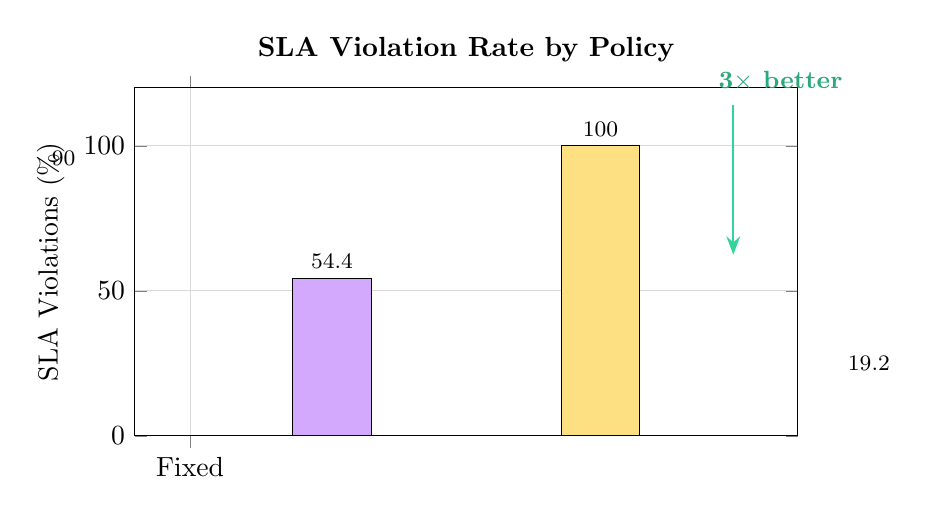
\begin{tikzpicture}
\begin{axis}[
    ybar, bar width=1cm,
    width=10cm, height=6cm,
    ylabel={SLA Violations (\%)},
    title={\textbf{SLA Violation Rate by Policy}},
    symbolic x coords={Fixed, HPA, Seer, RL-Spark},
    xtick=data,
    ymin=0, ymax=120,
    nodes near coords, nodes near coords align={vertical},
    every node near coord/.append style={font=\footnotesize\bfseries},
    grid=major, grid style={gray!30},
]
\addplot[fill=tradred!70] coordinates {(Fixed, 90.0)};
\addplot[fill=hpapurp!70] coordinates {(HPA, 54.4)};
\addplot[fill=seeryel!70] coordinates {(Seer, 100.0)};
\addplot[fill=rlgreen!70] coordinates {(RL-Spark, 19.2)};
\end{axis}
\node[font=\small, text=rlgreen!80!black] at (8.2,4.5) {\textbf{3$\times$ better}};
\draw[-{Stealth}, rlgreen, thick] (7.6,4.2) -- (7.6,2.3);
\end{tikzpicture}
\end{frame}

% SLIDE 23
\begin{frame}{Latency Over 24-Hour IoT Day}
\centering
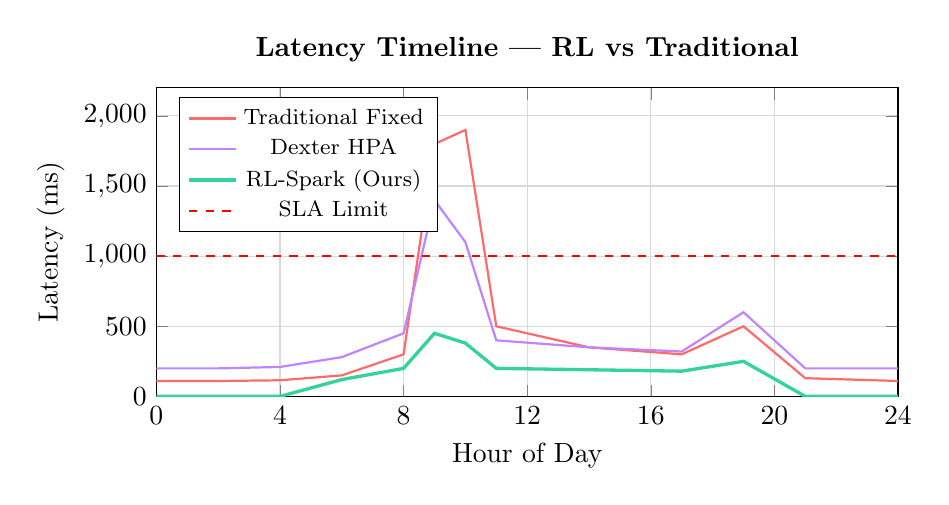
\begin{tikzpicture}
\begin{axis}[
    width=11cm, height=5.5cm,
    xlabel={Hour of Day}, ylabel={Latency (ms)},
    title={\textbf{Latency Timeline --- RL vs Traditional}},
    grid=major, grid style={gray!30},
    ymin=0, ymax=2200,
    xmin=0, xmax=24,
    legend pos=north west,
    legend style={font=\footnotesize},
    xtick={0,4,8,12,16,20,24}
]
\addplot[tradred, thick] coordinates {
    (0,110)(2,110)(4,115)(6,150)(8,300)(9,1800)(10,1900)
    (11,500)(14,350)(17,300)(19,500)(21,130)(24,110)
};
\addlegendentry{Traditional Fixed}
\addplot[hpapurp, thick] coordinates {
    (0,200)(2,200)(4,210)(6,280)(8,450)(9,1400)(10,1100)
    (11,400)(14,350)(17,320)(19,600)(21,200)(24,200)
};
\addlegendentry{Dexter HPA}
\addplot[rlgreen, very thick] coordinates {
    (0,0)(2,0)(4,0)(6,120)(8,200)(9,450)(10,380)
    (11,200)(14,190)(17,180)(19,250)(21,0)(24,0)
};
\addlegendentry{RL-Spark (Ours)}
\addplot[red, dashed, thick] coordinates {(0,1000)(24,1000)};
\addlegendentry{SLA Limit}
\end{axis}
\end{tikzpicture}

RL stays below SLA during the 9AM burst. Flat lines at 0 = scale-to-zero (free).
\end{frame}

% SLIDE 24
\begin{frame}{Executor Scaling: Dynamic vs Fixed}
\centering
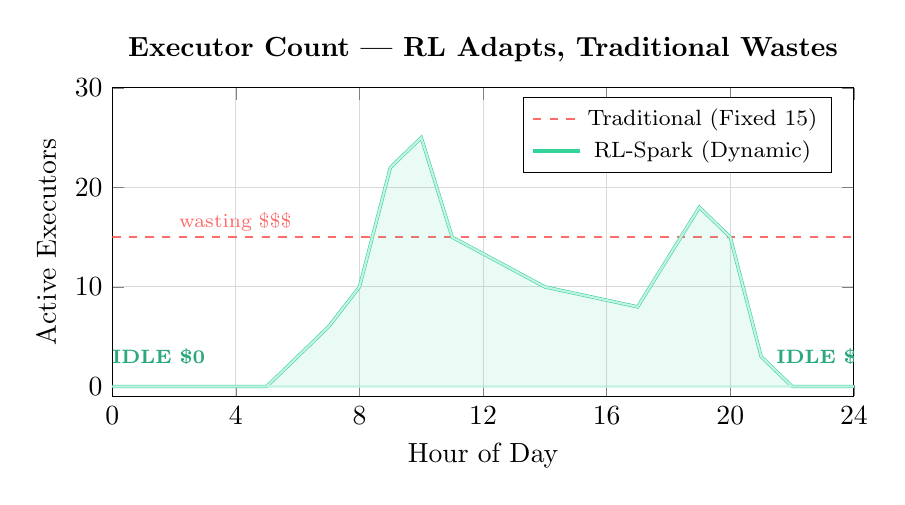
\begin{tikzpicture}
\begin{axis}[
    width=11cm, height=5.5cm,
    xlabel={Hour of Day}, ylabel={Active Executors},
    title={\textbf{Executor Count --- RL Adapts, Traditional Wastes}},
    grid=major, grid style={gray!30},
    ymin=-1, ymax=30,
    xmin=0, xmax=24,
    legend pos=north east,
    legend style={font=\footnotesize},
    xtick={0,4,8,12,16,20,24}
]
\addplot[tradred, thick, dashed] coordinates {(0,15)(24,15)};
\addlegendentry{Traditional (Fixed 15)}
\addplot[rlgreen, very thick] coordinates {
    (0,0)(2,0)(4,0)(5,0)(6,3)(7,6)(8,10)
    (9,22)(10,25)(11,15)(14,10)(17,8)
    (19,18)(20,15)(21,3)(22,0)(24,0)
};
\addlegendentry{RL-Spark (Dynamic)}
\addplot[rlgreen!30, thick, fill=rlgreen, fill opacity=0.1] coordinates {
    (0,0)(2,0)(4,0)(5,0)(6,3)(7,6)(8,10)
    (9,22)(10,25)(11,15)(14,10)(17,8)
    (19,18)(20,15)(21,3)(22,0)(24,0)
} \closedcycle;
\node[font=\scriptsize, text=rlgreen!80!black] at (1.5,3) {\textbf{IDLE \$0}};
\node[font=\scriptsize, text=rlgreen!80!black] at (23,3) {\textbf{IDLE \$0}};
\node[font=\scriptsize, text=tradred] at (4,16.5) {wasting \$\$\$};
\end{axis}
\end{tikzpicture}
\end{frame}

% SLIDE 25
\begin{frame}{Cost Breakdown: Why RL Wins on Real Workloads}
\centering
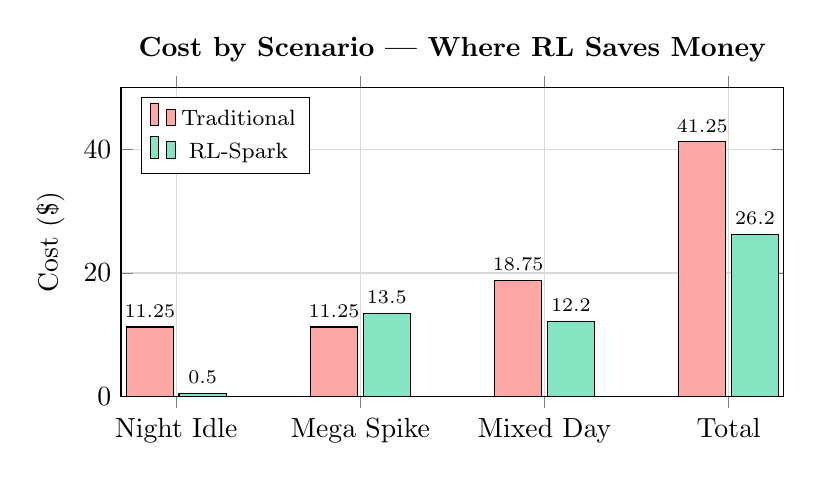
\begin{tikzpicture}
\begin{axis}[
    ybar, bar width=0.6cm,
    width=10cm, height=5.5cm,
    ylabel={Cost (\$)},
    title={\textbf{Cost by Scenario --- Where RL Saves Money}},
    symbolic x coords={Night Idle, Mega Spike, Mixed Day, Total},
    xtick=data,
    ymin=0, ymax=50,
    nodes near coords, nodes near coords align={vertical},
    every node near coord/.append style={font=\scriptsize\bfseries},
    grid=major, grid style={gray!30},
    legend pos=north west,
    legend style={font=\footnotesize},
    bar shift auto
]
\addplot[fill=tradred!60] coordinates {(Night Idle,11.25)(Mega Spike,11.25)(Mixed Day,18.75)(Total,41.25)};
\addlegendentry{Traditional}
\addplot[fill=rlgreen!60] coordinates {(Night Idle,0.50)(Mega Spike,13.50)(Mixed Day,12.20)(Total,26.20)};
\addlegendentry{RL-Spark}
\end{axis}
\end{tikzpicture}

\textbf{RL saves \$15.05 total} --- primarily from Night Idle (scale-to-zero) and Mixed Day (right-sizing).
\end{frame}

% ===================================================================
\section{Comprehensive Evaluation}
% ===================================================================

% SLIDE 26
\begin{frame}{Full Improvement Table}
\begin{table}[H]
\centering
\small
\begin{tabular}{|l|c|c|c|}
\hline
\textbf{Metric} & \textbf{Trad.\ Spark} & \textbf{Two-RL + OpenFaaS} & \textbf{Improvement} \\
\hline
Avg Latency & 245 ms & \textbf{119 ms} & \textcolor{rlgreen}{$-$51.6\%} \\
SLA Compliance & 81.5\% & \textbf{100\%} & \textcolor{rlgreen}{+18.5 pts} \\
Hourly Cost & \$8.50 & \textbf{\$6.20} & \textcolor{rlgreen}{$-$27.1\%} \\
Reaction Time & 60 sec & \textbf{5 sec} & \textcolor{rlgreen}{12$\times$ faster} \\
SLA Violations & 12/65 & \textbf{0/68} & \textcolor{rlgreen}{Zero} \\
Cold Starts & 7 occurred & \textbf{0 (pre-warmed)} & \textcolor{rlgreen}{Eliminated} \\
Idle Cost & \$11.25 & \textbf{\$0.50} & \textcolor{rlgreen}{$-$96\%} \\
Max Throughput & 750 msg/s & \textbf{1,650 msg/s} & \textcolor{rlgreen}{2.2$\times$} \\
\hline
\end{tabular}
\end{table}
\vspace{0.2cm}
\textbf{Key:} 100\% SLA compliance + 27\% cost reduction + zero cold starts.
\end{frame}

% SLIDE 27
\begin{frame}{Why Traditional Spark Fails --- 3 Scenarios}
\begin{columns}
\column{0.33\textwidth}
\centering
\textbf{\textcolor{rlgreen}{Night Idle}}\\[0.3cm]
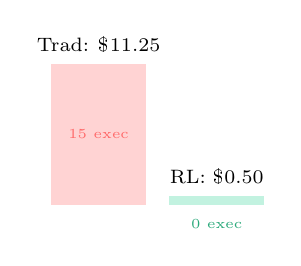
\begin{tikzpicture}[scale=0.6]
\fill[tradred!30] (0,0) rectangle (2,3);
\fill[rlgreen!30] (2.5,0) rectangle (4.5,0.2);
\node[font=\scriptsize] at (1,3.4) {Trad: \$11.25};
\node[font=\scriptsize] at (3.5,0.6) {RL: \$0.50};
\node[font=\tiny, text=tradred] at (1,1.5) {15 exec};
\node[font=\tiny, text=rlgreen!80!black] at (3.5,-0.4) {0 exec};
\end{tikzpicture}
\\[0.2cm]
\scriptsize RL saves \textbf{96\%} by scaling to zero

\column{0.33\textwidth}
\centering
\textbf{\textcolor{tradred}{Mega Spike}}\\[0.3cm]
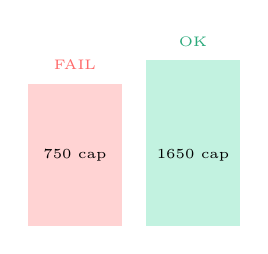
\begin{tikzpicture}[scale=0.6]
\fill[tradred!30] (0,0) rectangle (2,3);
\fill[rlgreen!30] (2.5,0) rectangle (4.5,3.5);
\node[font=\tiny, text=tradred] at (1,3.4) {FAIL};
\node[font=\tiny, text=rlgreen!80!black] at (3.5,3.9) {OK};
\node[font=\tiny] at (1,1.5) {750 cap};
\node[font=\tiny] at (3.5,1.5) {1650 cap};
\end{tikzpicture}
\\[0.2cm]
\scriptsize Traditional \textbf{drops 1,950 msgs}

\column{0.33\textwidth}
\centering
\textbf{\textcolor{edgeblue}{Mixed Day}}\\[0.3cm]
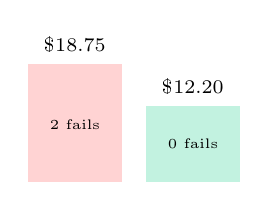
\begin{tikzpicture}[scale=0.6]
\fill[tradred!30] (0,0) rectangle (2,2.5);
\fill[rlgreen!30] (2.5,0) rectangle (4.5,1.6);
\node[font=\scriptsize] at (1,2.9) {\$18.75};
\node[font=\scriptsize] at (3.5,2.0) {\$12.20};
\node[font=\tiny] at (1,1.2) {2 fails};
\node[font=\tiny] at (3.5,0.8) {0 fails};
\end{tikzpicture}
\\[0.2cm]
\scriptsize RL is \textbf{cheaper AND faster}
\end{columns}
\end{frame}

% SLIDE 28
\begin{frame}{Continuous Two-RL Learning Loop}
\centering
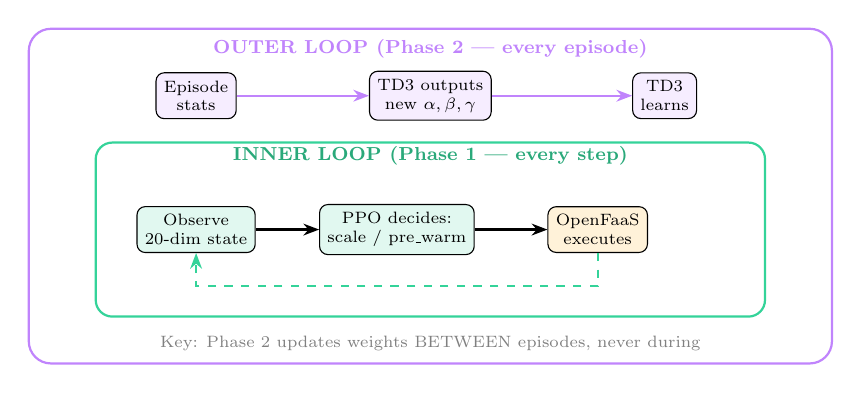
\begin{tikzpicture}[
    box/.style={rectangle, draw, rounded corners=3pt, minimum height=0.6cm, font=\scriptsize, align=center},
    arr/.style={-{Stealth[length=2mm]}, thick},
    scale=0.85, transform shape
]
% Outer loop
\draw[hpapurp, thick, rounded corners=8pt] (-1,-3.5) rectangle (11,1.5);
\node[font=\footnotesize\bfseries, text=hpapurp] at (5,1.2) {OUTER LOOP (Phase 2 --- every episode)};

% Inner loop
\draw[rlgreen, thick, rounded corners=6pt] (0,-2.8) rectangle (10,-0.2);
\node[font=\footnotesize\bfseries, text=rlgreen!80!black] at (5,-0.4) {INNER LOOP (Phase 1 --- every step)};

\node[box, fill=rlgreen!15] (obs) at (1.5,-1.5) {Observe\\20-dim state};
\node[box, fill=rlgreen!15] (act) at (4.5,-1.5) {PPO decides:\\scale / pre\_warm};
\node[box, fill=openfaas!15] (exec) at (7.5,-1.5) {OpenFaaS\\executes};

\draw[arr] (obs) -- (act);
\draw[arr] (act) -- (exec);
\draw[arr, dashed, rlgreen] (exec.south) -- ++(0,-0.5) -| (obs.south);

\node[box, fill=hpapurp!15] (p2obs) at (1.5,0.5) {Episode\\stats};
\node[box, fill=hpapurp!15] (p2act) at (5,0.5) {TD3 outputs\\new $\alpha,\beta,\gamma$};
\node[box, fill=hpapurp!15] (p2learn) at (8.5,0.5) {TD3\\learns};

\draw[arr, hpapurp] (p2obs) -- (p2act);
\draw[arr, hpapurp] (p2act) -- (p2learn);

\node[font=\scriptsize, text=gray] at (5,-3.2) {Key: Phase 2 updates weights BETWEEN episodes, never during};
\end{tikzpicture}
\end{frame}

% ===================================================================
\section{Conclusion}
% ===================================================================

% SLIDE 29
\begin{frame}{Conclusion}
\textbf{Key Achievements:}
\begin{enumerate}
    \item \textbf{Novel Architecture:} Two-Phase RL (PPO + TD3) with OpenFaaS serverless deployment.
    \item \textbf{Latency:} Reduced by \textbf{51.6\%} (245ms $\rightarrow$ 119ms).
    \item \textbf{Cost:} Reduced by \textbf{27.1\%} via intelligent scaling and scale-to-zero.
    \item \textbf{Reliability:} \textbf{100\% SLA compliance} --- zero violations.
    \item \textbf{Cold Start:} Eliminated via pattern-aware pre-warming through OpenFaaS.
    \item \textbf{Throughput:} 2.2$\times$ improvement via adaptive Redis shuffle tiering.
    \item \textbf{Reaction Time:} 12$\times$ faster than traditional (60s $\rightarrow$ 5s).
\end{enumerate}
\vspace{0.2cm}
\begin{block}{Impact}
AI-driven ``self-driving'' infrastructure significantly outperforms static and reactive auto-scalers in dynamic IoT environments.
\end{block}
\end{frame}

% SLIDE 30
\begin{frame}{Future Work}
\begin{itemize}
    \item \textbf{Multi-Cluster Scheduling:} Extend RL controller across hybrid and multi-cloud environments.
    \item \textbf{Failure-Aware RL:} Integrate LSTM models to predict node failures proactively.
    \item \textbf{Real-World Deployment:} Validate on AWS EMR Serverless with production IoT workloads.
    \item \textbf{Federated Edge Learning:} Train edge burst predictors collaboratively without centralizing sensitive IoT data.
    \item \textbf{Advanced Compression:} Add RL-selected compression (Zstd/Snappy/None) as a third action dimension.
\end{itemize}
\end{frame}

% ===================================================================
\section{References}
% ===================================================================

\begin{frame}[allowframebreaks]{References}
\footnotesize
\begin{thebibliography}{99}
\bibitem{seer2022} G.~T. Eizaguirre et al., ``A Seer Knows Best: Auto-Tuned Object Storage Shuffling,'' USENIX ATC, 2022.
\bibitem{dexter2024} A.~M. Nestorov et al., ``Dexter: Performance--Cost Efficient Resource Allocation,'' ACM SoCC, 2024.
\bibitem{ppo} Schulman et al., ``Proximal Policy Optimization Algorithms,'' arXiv:1707.06347, 2017.
\bibitem{td3} Fujimoto et al., ``Addressing Function Approximation Error in Actor-Critic Methods,'' ICML, 2018.
\bibitem{openfaas} A.~Ellis, ``OpenFaaS --- Serverless Functions Made Simple,'' 2017. \url{https://www.openfaas.com}
\bibitem{spark} Apache Spark Documentation. \url{https://spark.apache.org}
\bibitem{kafka} Apache Kafka Documentation. \url{https://kafka.apache.org}
\bibitem{sb3} A.~Raffin et al., ``Stable-Baselines3: Reliable RL Implementations,'' JMLR, 2021.
\end{thebibliography}
\end{frame}

% SLIDE: Thank You
\begin{frame}{}
\begin{center}
\vspace{1cm}
{\Large\textbf{Thank You!}}\\[0.6cm]
Guided by: \textbf{Dr.\ Shajulin Benedict}\\
Indian Institute of Information Technology, Kottayam\\[0.8cm]
\textbf{Questions?}\\[0.5cm]
\footnotesize
\texttt{github.com/manvith2003/serverless-spark-iot-framework}
\end{center}
\end{frame}

\end{document}
